\documentclass{article}

\usepackage{geometry}
\usepackage{amsmath}
\usepackage{graphicx, eso-pic}
\usepackage{listings}
\usepackage{hyperref}
\usepackage{multicol}
\usepackage{fancyhdr}
\pagestyle{fancy}
\fancyhf{}
\hypersetup{ colorlinks=true, linkcolor=black, filecolor=magenta, urlcolor=cyan}
\geometry{ a4paper, total={170mm,257mm}, top=10mm, right=20mm, bottom=20mm, left=20mm}
\setlength{\parindent}{0pt}
\setlength{\parskip}{0.3em}
\renewcommand{\headrulewidth}{0pt}

\rfoot{\thepage}
\fancyhf{} % sets both header and footer to nothing
\renewcommand{\headrulewidth}{0pt}
\lfoot{\textbf{CnC Intern Contest}}
\pagenumbering{gobble}

\fancyfoot[CE,CO]{\thepage}
\lstset{
    basicstyle=\ttfamily\small,
    columns=fixed,
    extendedchars=true,
    breaklines=true,
    tabsize=2,
    prebreak=\raisebox{0ex}[0ex][0ex]{\ensuremath{\hookleftarrow}},
    frame=none,
    showtabs=false,
    showspaces=false,
    showstringspaces=false,
    prebreak={},
    keywordstyle=\color[rgb]{0.627,0.126,0.941},
    commentstyle=\color[rgb]{0.133,0.545,0.133},
    stringstyle=\color[rgb]{01,0,0},
    captionpos=t,
    escapeinside={(\%}{\%)}
}

\begin{document}

\begin{center}

    
    \section*{Ke Rumah Pacar} % ganti judul soal

    \begin{tabular}{ | c c | }
        \hline
        Batas Waktu  & 1s \\    % jangan lupa ganti time limit
        Batas Memori & 256MB \\  % jangan lupa ganti memory limit
        \hline
    \end{tabular}
\end{center}

\subsection*{Deskripsi}
Adi adalah seorang yang setia. Ia memiliki pacar yang bernama Rani. Adi dan Rani tinggal di negara Aragen. Negara Aragen memiliki N kota dan M buah jalan. Setiap jalan memiliki panjang sendiri. Adi tinggal di kota Ida dan Rani tinggal di kota Inar. Untuk mengunjungi Rani, Adi akan menempuh perjalanan dengan jarak tempuh paling dekat. \\

Akan tetapi, untuk K hari kedepan akan terdapat perbaikan jalan diantara kota A dan kota B yang mengakibatkan Adi tidak dapat melewati jalan tersebut. Bantulah Adi untuk mencari jalan terdekat pada K hari tersebut

\subsection*{Format Masukan}

Baris pertama terdiri dari 4 bilangan bulat positif $N$, $M$, $a$, dan $b$ yang masing masing menyatakan banyak kota, banyak jalan, nomor kota Ida, dan Nomor kota Inar.\\
$M$ baris berikutnya berisi $U$, $V$, dan $W$ yang menyatakan bahwa ada jalan yang menghubungkan kota $U$ dan kota $V$ dengan panjang jalan $W$.\\
Baris selanjutnya terdiri dari 1 bilangan positif $Q$ yang menyatakan banyak query.\\
$Q$ baris selanjutnya terdiri dari 1 bilangan bulat positif $E$ dan $F$ yang menyatakan bahwa jalan antara kota $E$ dan kota $F$ pada hari tersebut rusak.\\ 
Hanya terdapat 1 jalan di antara 2 kota.
Perbaikan jalan pada 1 hari akan selesai sebelum hari selanjutnya. Artinya, perbaikan jalan hari ini akan bagus pada hari selanjutnya.


\subsection*{Constraint}
$1 \leq n \leq 2000$, $1 \leq m \leq 100.000$\\
$1 \leq a,b \leq n$\\
$1 \leq w \leq 100.000$\\
\subsection*{Format Keluaran}

Keluarkan K baris yang berisi jarak tercepat antara kota Ida dan kota Inar. Keluarkan -1 apabila tidak ada jalan antara kota Ida dan kota Inar.
\begin{multicols}{2}
\subsection*{Contoh Masukan}
\begin{lstlisting}
5 6 1 5
1 2 1
2 3 3
2 5 100
3 4 3
3 5 5
4 5 3
3
1 2
2 3
3 5
\end{lstlisting}
\columnbreak
\subsection*{Contoh Keluaran}
\begin{lstlisting}
-1
101
10
\end{lstlisting}
\vfill
\null
\end{multicols}





\pagebreak
\subsection*{Penjelasan}
\begin{center}
 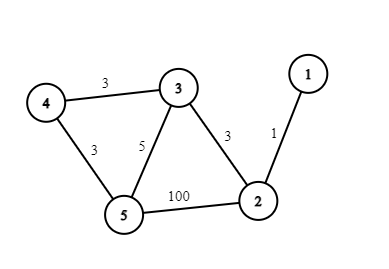
\includegraphics[scale=1.0]{graph_shortest.png}

\end{center}
Kita tahu bahwa kota Ida bernomor 1 dan kota Inar bernomor 5.\\
Pada hari pertama, tidak ada jalan antara kota Ida dan Inar. Sehingga outpunya -1\\
Pada hari kedua, jalan yang paling cepat adalah melewati kota $1 \rightarrow 2 \rightarrow 5$ sehingga jarak yang ditempuh adalah 101.\\ 
Pada hari ketiga, jalan yang paling cepat adalah melewati kota $1 \rightarrow 2 \rightarrow 3 \rightarrow 4 \rightarrow 5$ sehingga jarak yang ditempuh adalah 10.



\end{document}